\documentclass[a4paper,12pt]{article}
\usepackage[utf8]{inputenc}
\usepackage[T1]{fontenc}
\usepackage[english]{babel}
\usepackage{geometry}
\usepackage{color}
\usepackage{hyperref}
\usepackage{abstract}
\usepackage{multicol}
\usepackage{cite}
\hypersetup{
colorlinks,
citecolor=black,
filecolor=black,
linkcolor=black,
urlcolor=black
}
%\usepackage{tikz}
\usepackage{amsmath}
\usepackage{graphicx}
\usepackage{wrapfig}
\usepackage{subfigure}
\usepackage{fancyhdr} 
\usepackage{siunitx}

\title{\LARGE{\bf Traffic congestion prediction}}

%\author{\textit{Nico Curti, Rachele Luzi}}


\pagestyle{fancy}
\lhead{\textsf{\small Università di Bologna - Dipartimento di Fisica e Astronomia}}
\rfoot{\thepage}
\cfoot{}
\renewcommand{\headrulewidth}{0.4pt}

\begin{document}
\maketitle
\thispagestyle{fancy}
\rule[0.2cm]{13.5cm}{0.2mm}

\begin{abstract}
One of the main topics in complex systems studies concerns the traffic congestion prediction as a consequence of the increasing number of vehicles. We propose a novel pipeline to classify slowdowns situations processing data by the analysis of the features related to the fundamental diagram of traffic. We train a deep learning neural network providing a forewarning time of prediction related to the training set size. Then we compare our performances with those of the most common classifiers used in machine learning analysis. 

%\emph{With the increasing of vehicle population the problem the traffic behavior becomes one of central topics in complex systems studies. One of bigger problem is the traffic congestion prediction. We propose a novel pipeline to process traffic data with the aim to classify slowdowns situations. We analyze features related to the fundamental diagram of traffic and we identify a congestion close to a growing of density and a decreasing of flow cars. In order to predict slowdowns situation we binarize features and we train a deep learning neural network. We also compare the performances of a deep learning approach to the most common classifiers used in machine learning analysis. We obtain efficient predictions in the (\%) of analyzed dataset with a theoretical forewarning time of prediction till 30 minutes.}


%Traffic behavior prediction is fundamental to alleviate traffic congestions. We propose to classify the slowdowns situations analyzing the fundamental diagram of traffic
%which gives a relation between the traffic flow and the traffic density. A traffic congestion
%occurs when the density of the road grows up and the flow decreases. In order to predict
%congestion situations, we train the Replicated Focusing Belief Propagation architecture processing data according to the fundamental diagram of traffic.
\end{abstract}
\section{Introduction}
Understanding the daily traffic evolution is a fundamental actual topic since traffic congestions have become an integral part of our modern life and are cause of wasted fuel, air pollution and billions of wasted dollars in each year. It induces people to plan more time when travel bringing longer trip times and affecting the quality of life. Therefore research is attempting to handle this problem
or at least ease its adverse effects \cite{ZCW14,YB15}, also from the artificial intelligence point of view \cite{TG06, NT04, YR06, TMP07, SAB08}. There are several research methods used in the field of traffic prediction like deterministic, non-deterministic and stochastic \cite{C03} methods. Traditional studies have developed simulation techniques to model traffic congestion dynamics \cite{K13}, but many approaches have limitations, mainly due to errors during the calibration process of parameters and unrealistic assumptions. Besides the classification, our approach trains a deep learning algorithm to forecast traffic slowdowns and provide a forewarning time of prediction. 

Deep learning techniques \cite{NC11} are considered some of the most promising techniques to process huge high-dimensional data. The Binary Committee Machine Replicated Focusing Belief Propagation neural network (RFBP) is an iterative message-passing method that can be used to
describe a probability distribution over an instance described by a factor graph in the correlation decay approximation. We use this method with binary inputs which have been obtained by a collection of traffic road data. Data have been recorded by loop magnetic traffic detectors provided by Emilia Romagna region. Detectors record every car passing and generate an high time resolutions amount of data.

Many studies have been performed to estimate the urban traffic congestion and to implement prediction methods \cite{VKG14,HA15,ER15,DXSZ15,YDL15, CHW11, LYHVS11, PWM08}, focusing on various different features of classification. We present a method which is based on the study of the evolution of traffic flow, density and speed which are related through the fundamental diagram of traffic.  

The rest of the paper is organized as follows. The second section presents a description of the dataset and of our method of prediction. The third section describes our performances results making a comparison with other common classifiers. The fourth section concludes the paper.

\section{Materials and Method}
In this section, we describe the set of the data we deal with and our congestion prediction method, which involves the analysis of the fundamental diagram of traffic.

In order to effectively train the model to make forecasts under regular-congestion conditions which rise from car and road situations, a big set of past data is necessary for analysis. The car data have been collected by Emilia Romagna region over a period of one month (May 2011). The data are measured every time a car overcross a detector which records round-the-clock timestamp informations about direction, lane and driving speed. Processing mentioned data, we focus on two car dynamics features: the traffic flow and the vehicle density which are related according to the fundamental diagram of traffic (Figure \ref{diagram}) in homogeneous steady conditions.
Such quantities are defined as a function of a fixed number of cars: ...  which drive in a time interval and as the product between the flow and the car speed.

In order to avoid traffic congestion and to keep the traffic flow stable, the number of vehicles that enter the road must be smaller or equal than the number of vehicles that leaves it. At low traffic densities, where interactions among vehicles are rare, the flow grows nearly linearly with the density until a critical density value is reached, at which the flow reaches the road capacity taking its maximum value. In this situation the flow decreases as the density increases producing a queue of cars (figure \ref{densityflow}). 

%In figure \ref{diagram} we can visualize different traffic behaviors: we show the fundamental diagrams with respect two different daily situations. 

We first preprocess the data in order to eliminate noisy sample points, of which perceived positions are not consistent. In the second step we have to digitalize our signal according to the informations coming from the fundamental diagram structure. This is due to the theoretical model linked to the RFBP \cite{BB16, BB15} which can be used to derive marginal probabilities on a system within the Bethe-Peierls approximation and works with binarized input arrays. It is not well understood how this deep learning method is able to learn and how it doesn't get trapped in configurations with low computational performance. In order to classify slowdowns we apply a fuzzy binarization to the data and we associate to each car the value $-1$ or $+1$ as follows. We identify a slowdown occurrence when the road density is greater than the daily average road density and the traffic flow is decreasing. 
Using this definition we binarize the informations associating to each car the number $+ 1$ if it is involved in a slowdown either $-1$.
Thirdly we split each daily sequence into subsets of arbitrary length which produce a different time interval of prediction. Up to now we label each subset applying a majority rule to the values of the following subarray. In figure \ref{binary} we represent an example of the results of our processing. We highlight in the first two panels time regions of traffic flow and density which are responsible of congestion situations, then we represent in the third graph the result of our labelling \textbf{(sistemare bene l'ultima frase)}. 


\begin{figure}
\centering
\subfigure[01/05/2011]
{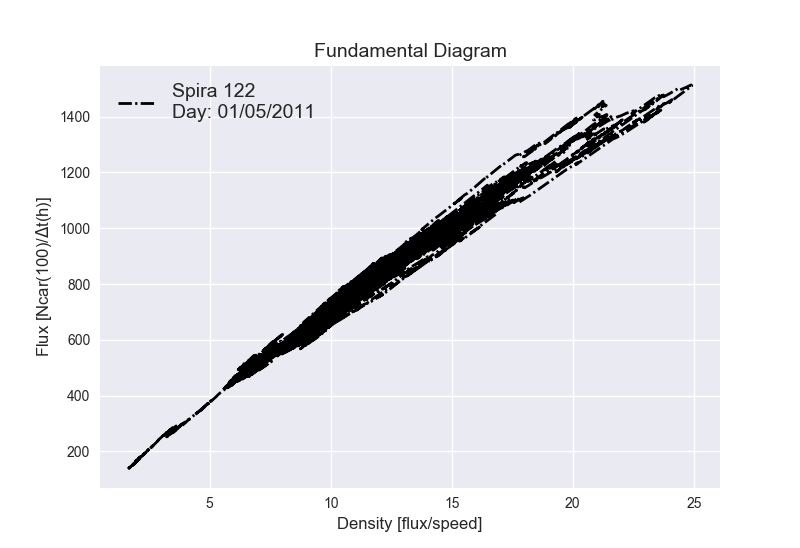
\includegraphics[width=5cm]{./images/diagram1.png}}
\hspace{1mm}
\subfigure[02/05/2011]
{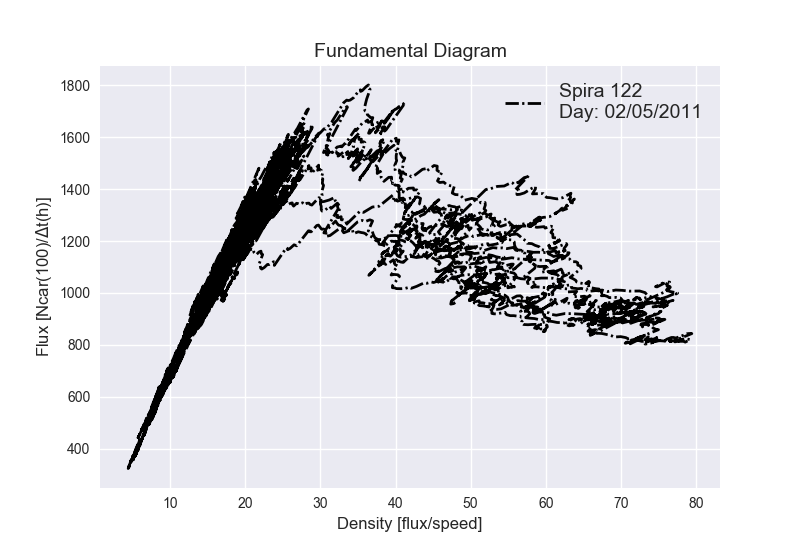
\includegraphics[width=5cm]{./images/diagram2.png}}
\caption{Fundamental diagrams. Left panel: uncongested day, the diagram present a linear behavior. The flow grows linearly with the density of the road without reaching the critical point so that it can be approximated by the density. Right panel: congested day, the diagram presents a cloud of points stemming from the line. After the road has reached its maximal capability, density continues to grow while the car speed, so the flow, decreases. }\label{diagram}
\end{figure}

\begin{figure}
\centering
\subfigure[01/05/2011]
{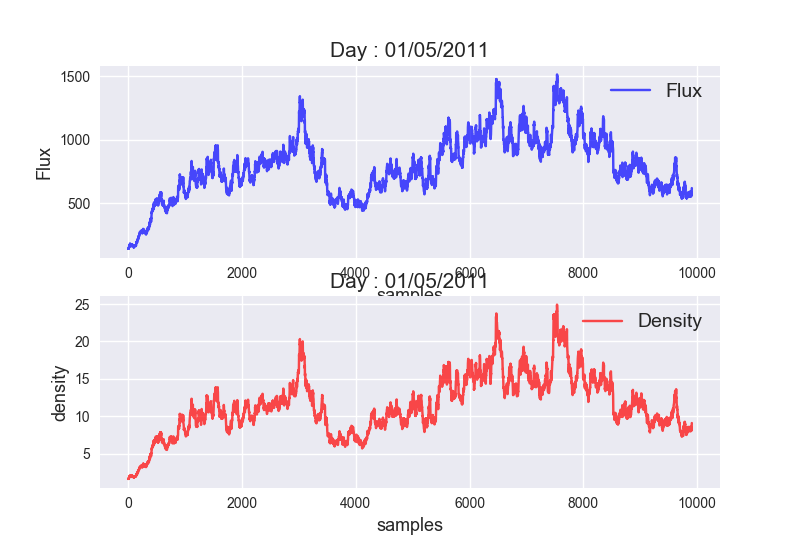
\includegraphics[width=5cm]{./images/density_flow1.png}}
\hspace{1mm}
\subfigure[02/05/2011]
{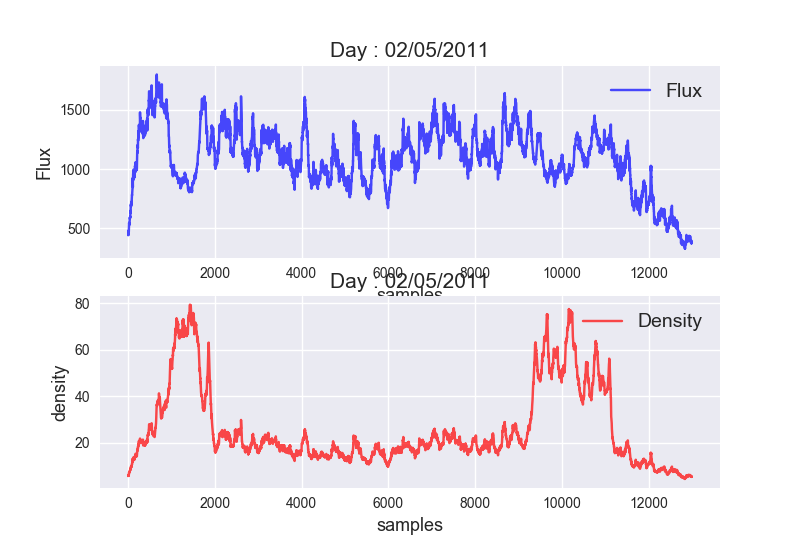
\includegraphics[width=5cm]{./images/density_flow2.png}}
\caption{Left panel: uncongested day, density and flow have a direct proportional behavior. Right panel: congested day, circled regions highlight congestion situations which occur when density increases and flow decreases.}\label{densityflow}
\end{figure}


\begin{figure}
{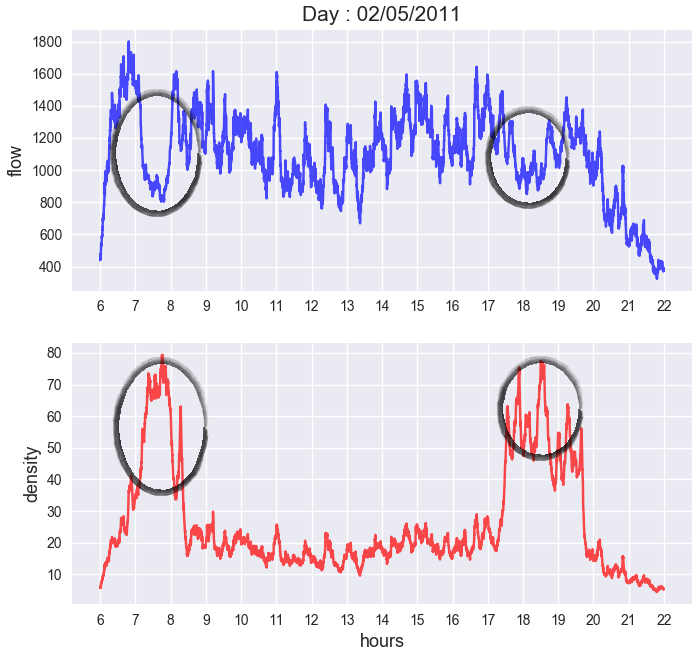
\includegraphics[width=5cm]{./images/density_flux_daily.png}}\quad
{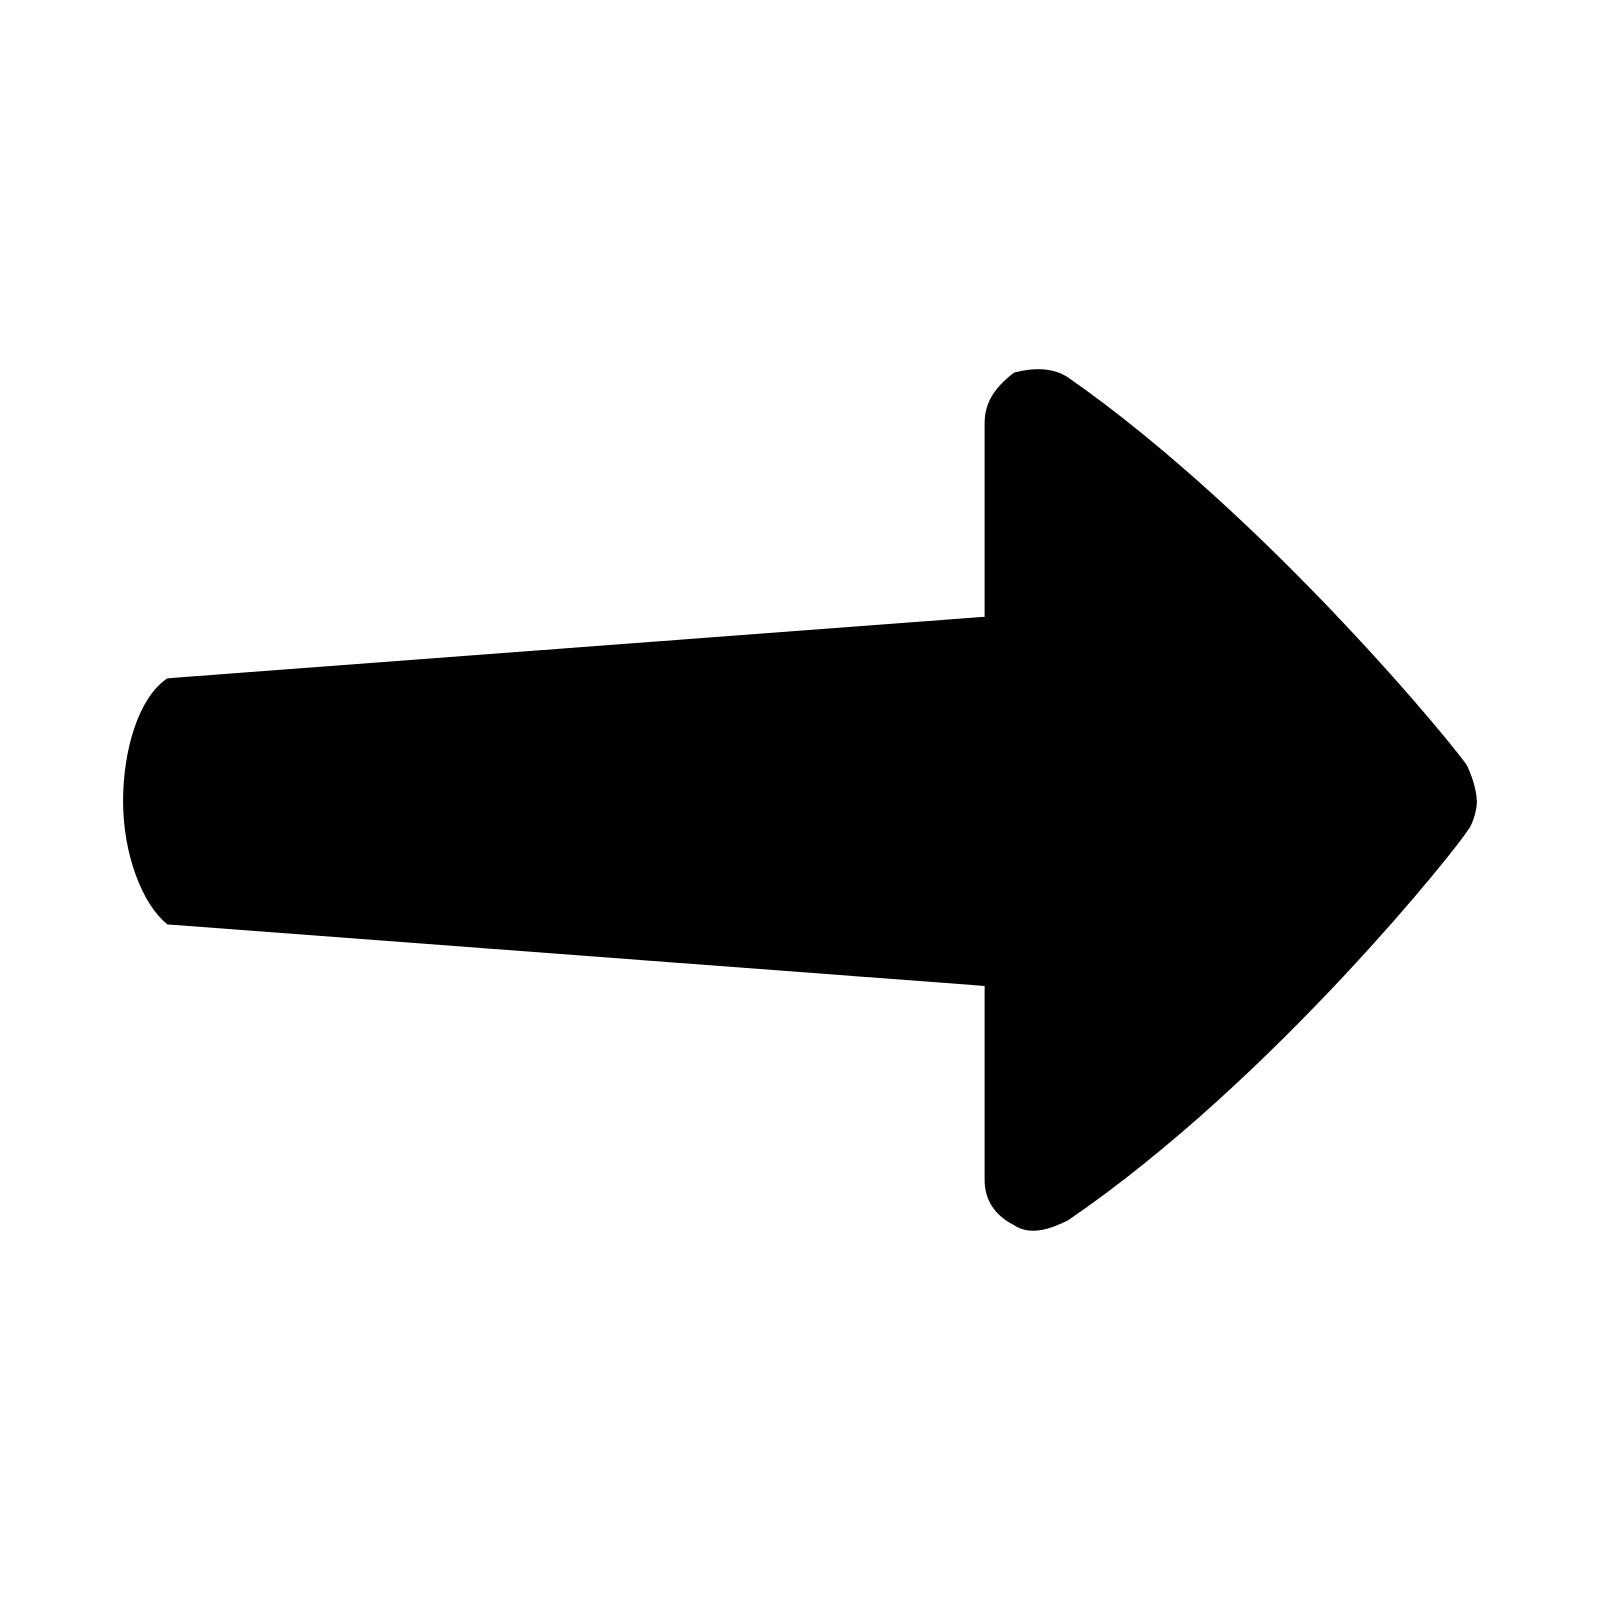
\includegraphics[width=2cm]{./images/r_arrow.png}}
{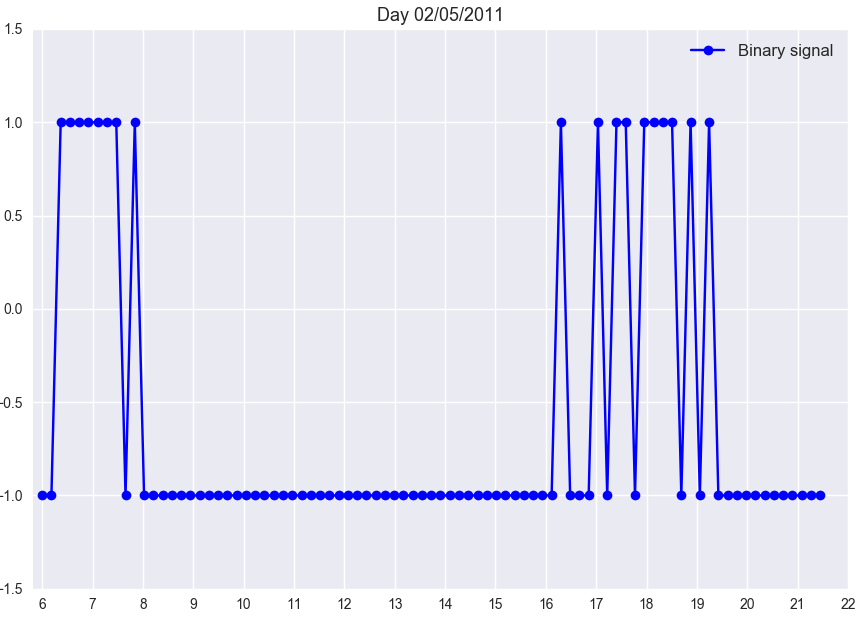
\includegraphics[width=5cm]{./images/binario.png}}
\caption{Results of binarization}\label{binary}
\end{figure}
\section{Results and Performances}
To benchmark our results and validate our approach, we compare our performances of prediction with those of ten other classifiers, namely KNeighbors (KNN), linear Support Vector Machine (lSVM), RBF Support Vector Machine (SVM), Gaussian Process, Decision Tree (DT), Random Forest (RF), MLP, AdaBoost (AB), Gaussian NB, QDA. 

As performances estimator we use the area under the receiver operating characteristic curve (AUC), i.e. the trapezoidal approximation of the area under the Receiver Operating Characteristic curve. The AUC corresponds to the probability that the classifier ranks a positive instance against a negative one. 
We represent in figure \ref{auc} the comparison of AUC values.
\begin{figure}
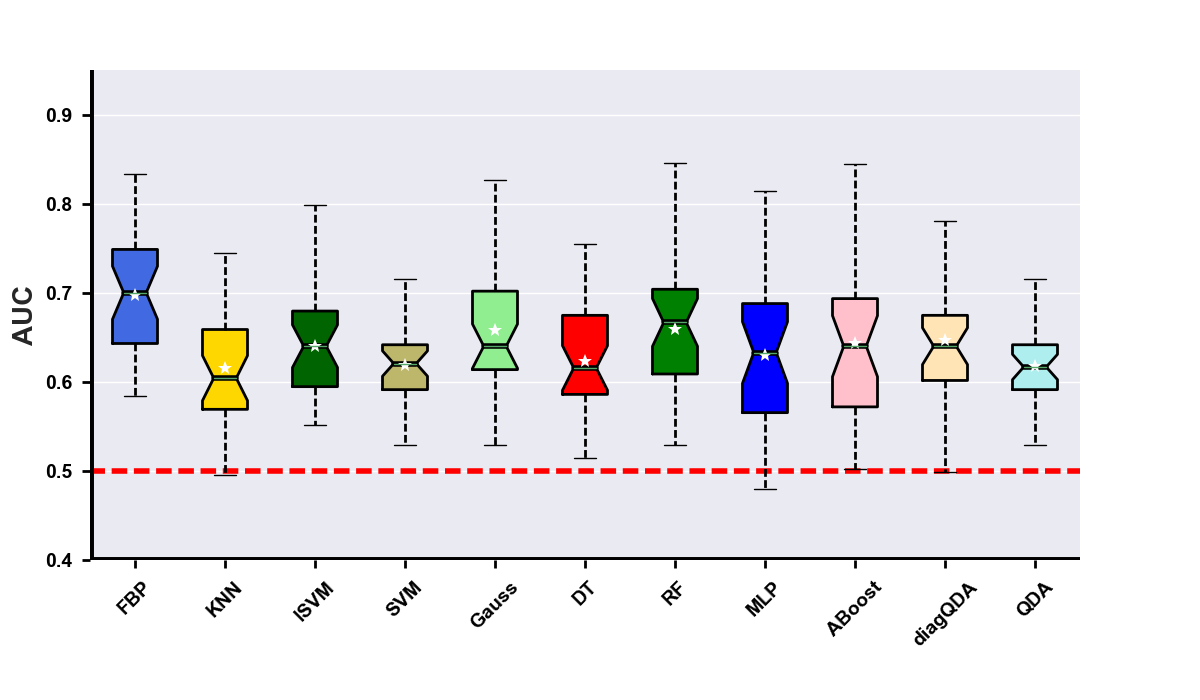
\includegraphics[scale=0.3]{./images/AUC_N201.png}
\caption{Comparison of AUC values.}\label{auc}
\end{figure}

Secondly we analyze the Matthew's Correlation Coefficient (MCC) which provides a balanced measure of the quality of binary classification taking into account true and false, positive and negatives even if classes have very different sizes. The MCC can take values in the range $[-1, +1]$.
The value +1 represent a total right classification, the value -1 a complete disagreement of prediction and the value 0 is associated to a random classifier.
We represent in figure \ref{mcc} the comparison of MCC values.
\begin{figure}
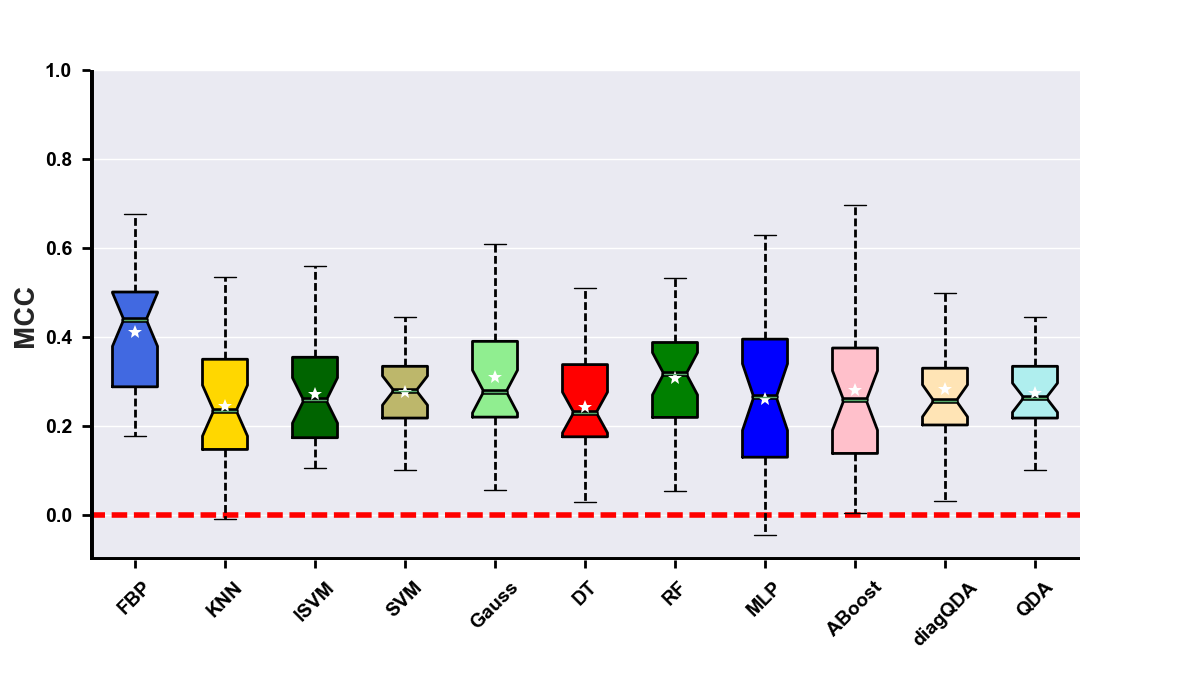
\includegraphics[scale=0.3]{./images/MCC_N201.png}
\caption{Comparison of MCC values.}\label{mcc}
\end{figure}

\begin{thebibliography}{4}
\bibitem{ZCW14} Y. Zheng, L. Capra, O. Wolfson, et al., \textit{Urban computing: concepts, methodologies,
and applications}, ACM Trans. Intell. Syst. Technol. 5 (3) 38, 2014.
\bibitem{YB15} M.B. Younes, A. Boukerche, A performance evaluation of an efficient traffic
congestion detection protocol (ECODE) for intelligent transportation systems,
Ad Hoc Netw. 24 317–336, 2015.

\bibitem{TG06} V. R. Tomás and L. A. Garcia, \textit{A Cooperative Multiagent System for Traffic Management
and Control}, The Fourth International Joint Conference on Autonomous Agents and
Multiagent Systems (AAMAS-06), 2006.
\bibitem{NT04} T. Nakata and J. Takeuchi, \textit{Mining Traffic Data from Probe-Car System for Travel Time
Prediction}, KDD’04, pp. 22-25, 2004.

\bibitem{YR06} X.-H. Yu and W. W. Recker, \textit{Stochastic adaptive control model for traffic signal systems},
Transportation Research Part C 14, pp. 263-282, Elsevier, 2006.
\bibitem{TMP07} K. Tufte, J. Li, D. Maier, V. Papadimos, R. L. Bertini, and J. Rucker, \textit{Travel Time
Estimation Using NiagaraST and latte}, SIGMOD’07, pp. 1091-1093, 2007.
\bibitem{SAB08} J.-D. Schmocker, S. Ahuja, and M. G. H. Bell, \textit{Multi-objective signal control of urban
junctions - Framework and a London case study}, Transportation Research Part C 16, pp.
454-470, 2008.

\bibitem{C03} E. Chung, \textit{Classification of traffic pattern}, Proceedings of the 11th World Congress on
ITS, 2003.

\bibitem{K13}S. Kurihara, \textit{Traffic-Congestion Forecasting Algorithm Based on Pheromone Communication Model}, Ant Colony Optimization - Techniques and Applications, Dr. Helio Barbosa (Ed.), InTech, DOI: 10.5772/52563, 2013.


\bibitem{NC11}J. Ngiam, A. Coates, A. Lahiri, B. Prochnow, Quoc V Le, and Andrew Y Ng, \textit{On optimization methods
for deep learning. In Proceedings of the 28th International Conference on Machine Learning} (ICML-11), pages 265–272,
2011.

\bibitem{VKG14}E. Vlahogianni, M. Karlaftis, and J. Golias, \textit{Short-term traffic forecasting: Where we are and where we're going},
Transportation Research Part C, vol. 43, Part 1, p. 3-19, June 2014.
\bibitem{HA15} H. Hashemi and K. F. Abdelghany, \textit{Real-time traffic network
state prediction for proactive traffic management},
Transportation Research Record, Journal of the Transportation
Research Board., vol. 2491, pp. 22–31, October 2015.
\bibitem{ER15} M. Elhenawy and H. A. Rakha, \textit{Automatic congestion
identification with two-component mixture models}, Transportation Research Record, Journal of the Transportation Research Board, vol. 2489, pp. 11–19, January 2015.
\bibitem{DXSZ15} C. Dong, Z. Xiong, C. Shao, and H. Zhang, \textit{A spatial temporal-based state space approach for freeway network traffic flow modelling and prediction}, Transportmetrica A: Transport Science. Taylor and Francis, vol. 11, no. 7, 2015.
\bibitem{YDL15} Y. Yuan, A. Duret, and H. van Lint, \textit{Mesoscopic traffic
state estimation based on a variational formulation of the lwr model in lagrangian-space coordinates and kalman filter},
Transportation Research Procedia, vol. 10, pp. 82–92, 2015.
\bibitem{CHW11} T. Cheng, J. Haworth, and J. Wang, \textit{Spatio-temporal autocorrelation
of road network data}, Journal of Geographical
Systems, vol. 14, no. 4, pp. 1–25, 2011.

\bibitem{LYHVS11} J. W. C. V. Lint, Y. Yuan, S. P. Hoogendoorn, J. L. M. Vrancken, and T. Schreiter, \textit{Freeway traffic state estimation
using extended kalman filter for first-order traffic model in
lagrangian coordinates}, Proceedings of the IEEE International Conference on Networking, Sensing and Control, ICNSC 2011, Delft, The Netherlands., 2011.
\bibitem{PWM08} M. Papageorgiou, Y. Wang, and A. Messmer, \textit{Real-time freeway traffic state estimation based on extended kalman
filter: adaptive capabilities and real data testing}, Transport. Research Part A: Policy Pract., vol. 42, no. 10, pp. 1340–1358, 2008.

\bibitem{BB16}C. Baldassi, C. Borgs, Jennifer Chayes, A.
Ingrosso, C. Lucibello, L. Saglietti, and R. Zecchina,\textit{Unreasonable Effectiveness of Learning Neural Networks: From Accessible States and
Robust Ensembles to Basic Algorithmic Schemes} vol. 113 no. 48,  E7655–E7662, doi: 10.1073/pnas.1608103113, 2016.

\bibitem{BB15} C. Baldassi and A. Braunstein, \textit{A Max-Sum algorithm for training discrete neural networks}, Journal of Statistical Mechanics: Theory and Experiment, no. 8, P08008, http://stacks.iop.org/1742-5468/2015/i=8/a=P08008, 2015.
\end{thebibliography}
\end{document}




